This section introduces our new vision of data integration, proposes our approach and briefly presents our query rewriting algorithm guided by user preferences and SLAs.

\subsection{New vision of Data Integration}

\begin{figure}[th!]
\center
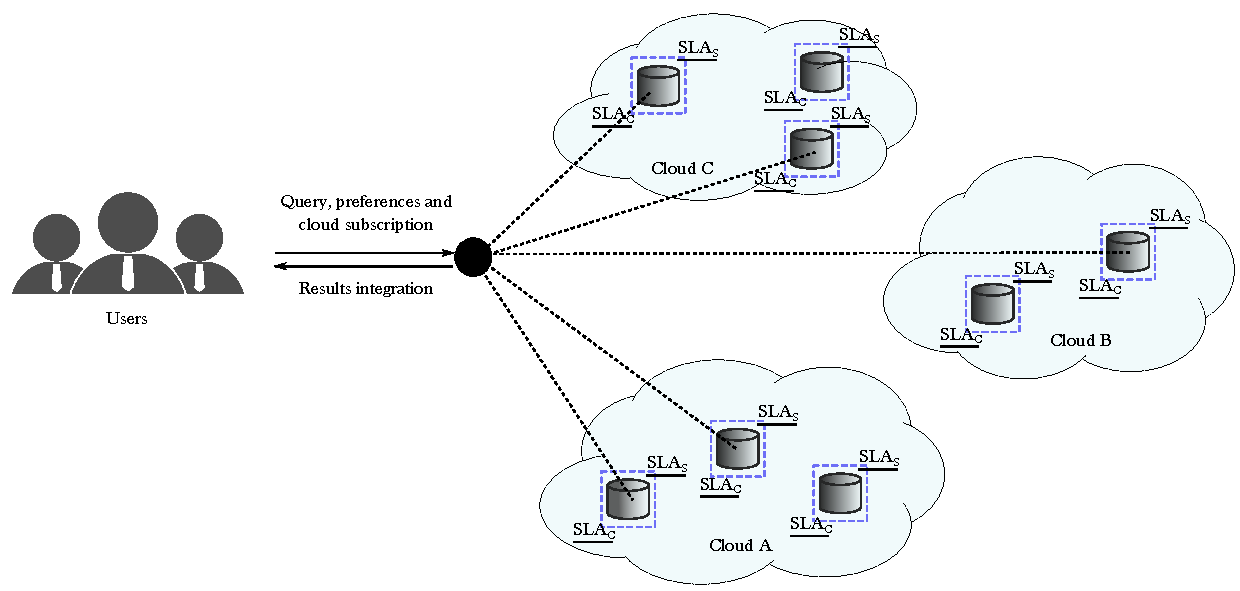
\includegraphics[scale=0.40]{scenario.pdf}
\caption{Data integration scenario}\label{fig:scenario}
\end{figure}

In our work, we consider a new vision of data integration in a multi-cloud context (see figure~\ref{fig:scenario}). Data is accessed and retrieved as \textit{data services} deployed in \textit{cloud providers} geographically distributed. \textit{Data services} and \textit{cloud providers} export their SLA specifying the level of services they can guarantee to users. Two types of SLA are considered: (1) cloud SLA (SLA$_{C}$), agreements between a \textit{data service} and a \textit{cloud provider}; and (2) service SLA (SLA$_{S}$), agreements between \textit{users} and \textit{data services}. The figure~\ref{fig:cloudsla} illustrates a cloud SLA schema.  

\begin{figure*}[th!]
\center
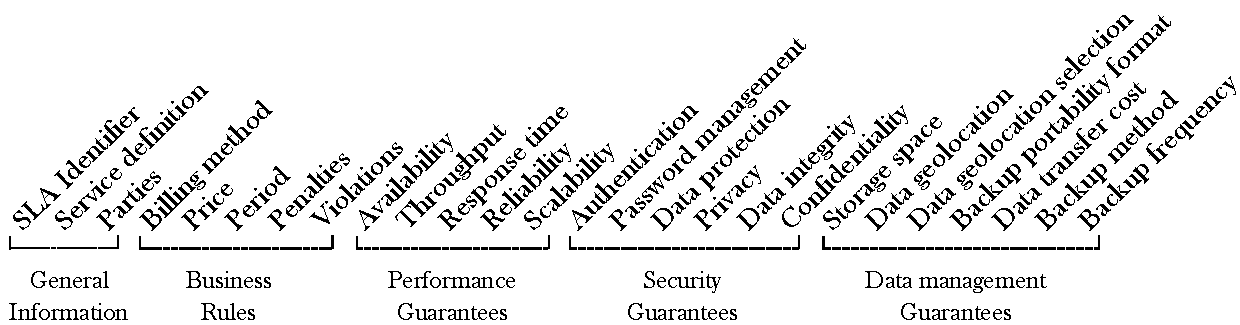
\includegraphics[scale=0.57]{Cloud_SLA.pdf}
\caption{Cloud SLA}\label{fig:cloudsla}
\end{figure*}

Therefore, given a user query, her integration quality requirements and her cloud subscription, it is rewritten in terms of cloud services (\textit{data services} and \textit{data processing services}) composition that fulfill the integration requirements and deliver the expected results to the user. This new vision brings challenges to data integration, such as:
\begin{itemize}
\item \textbf{Performance}. In the multi-cloud, we are dealing with a huge amount of \textit{data services}, \textit{data processing services} and \textit{cloud providers}. Consequently, producing and executing service compositions can require an important quantity of resources and processing time.
\item \textbf{Economic model}. Even with the possibility of having an unlimited access to resources, the user is limited to the resources she has contracted and to the budget she is ready to pay for. Thus, it is crucial to design new methods in order to produce rewritings which satisfies the user integration requirements and the cloud economic model. 
\item \textbf{Quality issues}. Some rewritings produced and executed to the user query could not satisfy her quality requirements concerning privacy, data provenance, cost, among others. Producing and executing these rewritings implies increasing time processing and integration total cost. 
\item \textbf{SLA heterogeneity}. While producing the rewritings, it is necessary to match the user requirements with the different SLAs exported by the \textit{cloud providers} and \textit{cloud services}. In the multi-cloud, \textit{cloud providers} and \textit{cloud services} export SLAs with different semantics and structure that makes the matching SLA and user requirement challenging. In addition, we are also dealing with incompatibilities of SLAs.
\item \textbf{Reuse}. Rewriting and executing the user query is computationally costly in terms of processing time and economic cost. Thus, it is necessary to propose a manner of reusing previous integration in order to save time and money, but also meeting the user expectations.
\end{itemize}

\subsection{SLA-based data integration approach}
Motivated by the challenges discussed in the previous section, we propose our SLA-based data integration approach to multi-cloud environments. The data integration process includes (i) looking up services that can be used as \textit{data services}, and for services required to process the retrieved data and build an integrated result (called \textit{data processing services}); (ii) processing data retrieval, processing and integration; and (iii) delivering results to the user considering her quality requirements, context and resource consumption.  In this sense, our approach is divided in four steps. Given a user \textit{query}, a set of user \textit{preferences} associated to it, \textit{cloud providers} and \textit{cloud services}:
\\
\textbf{\underline{SLA derivation}}. In this step, we compute what we call an \textsl{integrated
SLA} that matches (including quality constraints and data requirements) with the SLA's provided by \textit{cloud services}, given a specific user cloud subscription. The user may have general \textit{preferences} depending on the context she wants to integrate her data such as economic cost, bandwidth limit, free services, and storage and processing limits. The \textit{SLA derivation} is the big challenge while dealing with SLAs and particularly for adding quality dimensions to data integration. Furthermore, the \textsl{integrated SLA} guides the query evaluation, and the way results are computed and delivered. \\
\textbf{\underline{Filtering data services}}. The \textsl{integrated SLA} is used (i)
to filter previous SLA derived for a similar request in order to reuse previous results; or (ii) to filter possible \textit{cloud services} that can be used for answering the query. The SLA exported by a selected \textit{cloud service} should satisfy the user \textit{preferences}. \\
\textbf{\underline{Query rewriting}}. Given a set of \textit{data services} that can
potentially provide data for integrating the query result, a set of service compositions is generated according to the \textsl{integrated SLA} and the agreed SLA of each \textit{data services}. \\
\textbf{\underline{Integrating a query result}}. The service compositions are executed
in one or several clouds where the user has a subscription. The execution cost of service compositions must fulfill the \textsl{integrated SLA}. The clouds resources needed to execute the composition and how to use them is decided taking in consideration the economic cost determined by the data to be transferred, the number of external calls to services, data storage and delivery cost.

The algorithm 1 describes in general lines our approach which integrate data on multi-cloud environments considering quality aspects. Giver a user query $Q$, its associated user preferences $P$, a user integration context (its cloud subscription ($C$)), a set of previous \textit{integrated SLA} $\bigSLA$, a set of \textit{data services} ($DS$), a set of \textit{data processing services} ($DPS$) and a set of \textit{cloud providers} $CP$, the integration results ($IR$) is delivered to the user fulfilling her preferences and considering her integration context. The approach begins looking for previous \textit{integrated SLAs} that can be matched with the user query and user' preferences (lines 2 - 6). The set $pI$ includes all matched i (line 4). If previous \textit{integrated SLA} are identified (line 7), the one that perfectly matches with the user preferences is selected (line 8). Then, a new \textit{integrated SLA} is computed to user query based on the previous \textit{integrated SLA}, her preferences and her context (line 9). At this step, the services composition produced to a previous query is reused from its \textit{integrated SLA} ($sI$). Otherwise, a new \textit{integrated SLA} is created to user request given the query, the preferences and the context (line 11). Then, it is updated by calling the \textit{Rhone} procedure (line 12). The \textit{Rhone} is responsible (i) to select \textit{data services} (in $DS$) and \textit{data processing services} (in $DPS$) which satisfy the user preferences based on their SLAs; and (ii) to produce services compositions that completely match with the query and fulfill the user preferences. Finally, the integration results ($IR$) are produced and delivered to the user considering her context executing the service compositions generated to the user query (included in the \textit{integrated SLA}). Note that while executing compositions, it is necessary to satisfy the user context requirements and also to dynamically update the integrated SLA adding the information of contracts that were established to allow the integration. Finally, the integrated SLA is stored to be used in a next query.   

\begin{algorithm} 
%\small
\caption{ - SLA-based data integration}
\label{qualityBasedAlgorithm}
\begin{algorithmic}[1]
\REQUIRE Query ($Q$), user preferences ($P$), user cloud subscription ($C$) and a set of previous \textit{integrated SLA} ($\bigSLA$).
\ENSURE Integration results delivered considering the user context (cloud subscription).
%\STATE \textbf{function} $\mathit{SelectCandidateServices} (Q, \bigS)$
%\STATE let $\bigSLA$ be a set of previous integrated SLA
\STATE $pI \leftarrow \emptyset$
\FORALL  {$SLA_{i}$ in $\bigSLA$}
	\IF {$\mathit{macthes(Q, P, SLA_{i})}$}
		\STATE $pI \leftarrow pI \cup \lbrace SLA_{i} \rbrace$		
%		\FORALL  {$A_{j}$ in $S_{i}$}
%			\IF {$Q.\mathit{notContains(A_{i})}$}
%				\STATE $b \leftarrow \mathit{false}$	
%				\STATE $\mathit{break}$
%			\ENDIF
%		\ENDFOR
%		\IF {$b = true$}
%			\STATE $\bigLS \leftarrow \bigLS \cup \lbrace S_{i} \rbrace$	
%		\ENDIF
	\ENDIF
\ENDFOR
\IF {$pI \neq \emptyset$}
	\STATE $sI \leftarrow chooseBest(P, pI)$
	\STATE $newSLA_{i} \leftarrow deriveSLA(sI, P, C)$
%	\FORALL  {$SLA_{i}$ in $pI$}
%		\STATE $sI \leftarrow choose(P,)$
%	\ENDFOR
\ELSE
	\STATE $newSLA_{i} \leftarrow deriveSLA(Q, P, C)$
	\STATE $newSLA_{i} \leftarrow Rhone(newSLA_{i})$
\ENDIF
\STATE $IR \leftarrow execute(newSLA_{i})$
\STATE \textbf{return} $IR$
\STATE \textbf{end function}
\end{algorithmic}
\end{algorithm} 

\subsection{Query rewriting algorithm}
To serve as a proof of concept to our approach, we intend to develop a query
rewriting algorithm which is guided by users' integration requirements and
service level agreements exported by different data services and cloud
providers. The query rewriting is an important issue in data integration. In
cloud computing, researches have refereed to it as a service composition problem
in which given a query the objective is to lookup and compose data services that
can contribute to produce a result. \cite{Barhamgi2010} proposed a query
rewriting approach which processes queries on data provider services.
\cite{Benouaret2011} introduced a service composition framework to answer
preference queries. Two algorithms inspired on~\cite{Barhamgi2010} are presented
to rank the best rewritings based on previously computed scores. \cite{ba2014}
extended \cite{Umberto} and presented an refinement algorithm that produces and
order rewritings according to user preferences and scores. In general, these
works share the same performance problem depending on the size of the query and
on the number of available services. Furthermore, they do not take into
consideration user's integration requirements what can lead to produce
rewritings that are not satisfactory to the user in terms of quality
requirements and cost. Currently, we have formalized and developed a rewriting
algorithm that considers user preferences and services' quality aspects while
selecting services and producing rewritings called \textit{Rhone} (Invoked in the algorithm 1, line 12).                    